\documentclass[12pt]{article}
\usepackage[utf8]{inputenc}
\usepackage[T1]{fontenc}
\usepackage[spanish,es-lcroman]{babel}
\usepackage{amsmath}
\usepackage{amsthm}
\usepackage{amsfonts}
\usepackage{amssymb}
\usepackage{physics}
\usepackage{tikz}
\usepackage{float}
\usepackage{calc}
\usepackage[autostyle,spanish=mexican]{csquotes}
\usepackage[per-mode=symbol]{siunitx}
\usepackage{textcomp, gensymb}
\usepackage{multicol}
\usepackage{enumitem}
\usepackage{hyperref}
\usepackage{setspace}
\usepackage[left=2.00cm, right=2.00cm, top=2.00cm, 
     bottom=2.00cm]{geometry}
% \usepackage{Estilos/ColoresLatex}
\usepackage{makecell}
\usepackage{subcaption}
\usepackage[skip=10pt, indent=30pt]{parskip}
% \usepackage{scalerel}
\usepackage{scalerel}[2016-12-29]
\usepackage{biblatex}
\usepackage{cancel}
\usepackage{tcolorbox}
\usepackage{wrapfig}
\usepackage{multirow}

\definecolor{ao}{rgb}{0.0, 0.0, 1.0}

\hypersetup{
    colorlinks=true,
    linkcolor=ao,
    filecolor=magenta,      
    urlcolor=ao,
}

\newcommand{\ptilde}[1]{\ensuremath{{#1}^{\prime}}}
\newcommand{\stilde}[1]{\ensuremath{{#1}^{\prime \prime}}}
\newcommand{\ttilde}[1]{\ensuremath{{#1}^{\prime \prime \prime}}}
\newcommand{\ntilde}[2]{\ensuremath{{#1}^{(#2)}}}
\newcommand{\pderivada}[1]{\ensuremath{{#1}^{\prime}}}
\newcommand{\sderivada}[1]{\ensuremath{{#1}^{\prime \prime}}}
\newcommand{\tderivada}[1]{\ensuremath{{#1}^{\prime \prime \prime}}}
\newcommand{\nderivada}[2]{\ensuremath{{#1}^{(#2)}}}

\def\stretchint#1{\vcenter{\hbox{\stretchto[440]{\displaystyle\int}{#1}}}}
\def\scaleint#1{\vcenter{\hbox{\scaleto[3ex]{\displaystyle\int}{#1}}}}
\def\scaleiint#1{\vcenter{\hbox{\scaleto[6ex]{\displaystyle\iint}{#1}}}}
\def\scaleiiint#1{\vcenter{\hbox{\scaleto[6ex]{\displaystyle\iiint}{#1}}}}
\def\scaleoint#1{\vcenter{\hbox{\scaleto[3ex]{\displaystyle\oint}{#1}}}}
\def\bs{\mkern-12mu}

% \newcommand{\textbf}[2]{\textbf{\textcolor{#1}{#2}}}
\sisetup{per-mode=symbol}
\decimalpoint
\sisetup{bracket-numbers = false}
\newlength{\depthofsumsign}
\setlength{\depthofsumsign}{\depthof{$\sum$}}
\newcommand{\nsum}[1][1.4]{% only for \displaystyle
    \mathop{%
        \raisebox
            {-#1\depthofsumsign+1\depthofsumsign}
            {\scalebox
                {#1}
                {$\displaystyle\sum$}%
            }
    }
}

\AtBeginDocument{\RenewCommandCopy\qty\SI}
\ExplSyntaxOn
\msg_redirect_name:nnn { siunitx } { physics-pkg } { none }
\ExplSyntaxOff

\numberwithin{equation}{section}

\linespread{1.25}

\renewcommand{\labelenumii}{\theenumii}
\renewcommand{\theenumii}{\theenumi.\arabic{enumii}.}

\emergencystretch=1em
% \documentclass[hidelinks,12pt]{article}
\usepackage[left=0.25cm,top=1cm,right=0.25cm,bottom=1cm]{geometry}
%\usepackage[landscape]{geometry}
\textwidth = 20cm
\hoffset = -1cm
\usepackage[utf8]{inputenc}
\usepackage[spanish,es-tabla]{babel}
\usepackage[autostyle,spanish=mexican]{csquotes}
\usepackage[tbtags]{amsmath}
\usepackage{nccmath}
\usepackage{amsthm}
\usepackage{amssymb}
\usepackage{mathrsfs}
\usepackage{graphicx}
\usepackage{subfig}
\usepackage{standalone}
\usepackage[outdir=./Imagenes/]{epstopdf}
\usepackage{siunitx}
\usepackage{physics}
\usepackage{color}
\usepackage{float}
\usepackage{hyperref}
\usepackage{multicol}
%\usepackage{milista}
\usepackage{anyfontsize}
\usepackage{anysize}
%\usepackage{enumerate}
\usepackage[shortlabels]{enumitem}
\usepackage{capt-of}
\usepackage{bm}
\usepackage{relsize}
\usepackage{placeins}
\usepackage{empheq}
\usepackage{cancel}
\usepackage{wrapfig}
\usepackage[flushleft]{threeparttable}
\usepackage{makecell}
\usepackage{fancyhdr}
\usepackage{tikz}
\usepackage{bigints}
\usepackage{scalerel}
\usepackage{pgfplots}
\usepackage{pdflscape}
\pgfplotsset{compat=1.16}
\spanishdecimal{.}
\renewcommand{\baselinestretch}{1.5} 
\renewcommand\labelenumii{\theenumi.{\arabic{enumii}})}
\newcommand{\ptilde}[1]{\ensuremath{{#1}^{\prime}}}
\newcommand{\stilde}[1]{\ensuremath{{#1}^{\prime \prime}}}
\newcommand{\ttilde}[1]{\ensuremath{{#1}^{\prime \prime \prime}}}
\newcommand{\ntilde}[2]{\ensuremath{{#1}^{(#2)}}}

\newtheorem{defi}{{\it Definición}}[section]
\newtheorem{teo}{{\it Teorema}}[section]
\newtheorem{ejemplo}{{\it Ejemplo}}[section]
\newtheorem{propiedad}{{\it Propiedad}}[section]
\newtheorem{lema}{{\it Lema}}[section]
\newtheorem{cor}{Corolario}
\newtheorem{ejer}{Ejercicio}[section]

\newlist{milista}{enumerate}{2}
\setlist[milista,1]{label=\arabic*)}
\setlist[milista,2]{label=\arabic{milistai}.\arabic*)}
\newlength{\depthofsumsign}
\setlength{\depthofsumsign}{\depthof{$\sum$}}
\newcommand{\nsum}[1][1.4]{% only for \displaystyle
    \mathop{%
        \raisebox
            {-#1\depthofsumsign+1\depthofsumsign}
            {\scalebox
                {#1}
                {$\displaystyle\sum$}%
            }
    }
}
\def\scaleint#1{\vcenter{\hbox{\scaleto[3ex]{\displaystyle\int}{#1}}}}
\def\bs{\mkern-12mu}


%\usepackage{showframe}
\title{Funciones de Chebyshev \\ \large {Tema 5 - Funciones especiales} \vspace{-3ex}}
\author{M. en C. Gustavo Contreras Mayén}
\date{ }

\begin{document}
\maketitle
\fontsize{14}{14}\selectfont
\spanishdecimal{.}
\tableofcontents
\newpage

%Referencia Riley 18.4 Chebyshev functions
\section{Funciones de Chebyshev.}

La ecuación diferencial de Chebyshev tiene la forma:
\begin{align}
(1 - x^{2}) \, \sderivada{y} - x \, \pderivada{y} + \nu^{2} \, y
 = 0
 \label{eq:ecuacion_18_054}
\end{align}
y tiene tres puntos singulares regulares, en $x = -1, 1, \infty$. Al comparar la ecuación con:
\begin{align*}
(1 - x^{2}) \, \sderivada{y} - x \, \pderivada{y} + \ell (\ell + 1) \, y = 0
\end{align*}
%vemos que la ecuación de Chebyshev es muy similar en forma a la ecuación de Legendre. A pesar de esta similitud, l
La ecuación (\ref{eq:ecuacion_18_054}) no se presenta con mucha frecuencia en problemas físicos, aunque \emph{sus soluciones son de considerable importancia en el análisis numérico}.
\par
El parámetro $\nu$ es un número real dado, pero en casi todas las aplicaciones prácticas toma un valor entero. De aquí en adelante asumimos que $\nu = n$, donde $n$ es un número entero no negativo. %Como fue el caso de la ecuación de Legendre, 
En el uso normal la variable $x$ es el coseno de un ángulo, por lo que $-1 \leq x \leq 1$. Cualquier solución de la ec. (\ref{eq:ecuacion_18_054}) se llama \emph{función de Chebyshev}.
\par
El punto $x = 0$ es un punto ordinario de la ec. (\ref{eq:ecuacion_18_054}), por lo que esperamos encontrar
dos soluciones linealmente independientes de la forma:
\begin{align*}
y = \nsum_{m=0}^{\infty} a_{m} \, x^{m}
\end{align*}
Se podrían encontrar las relaciones de recurrencia para los coeficientes $a_{m}$, % de una manera similar a la utilizada para la ecuación de Legendre.
para la ecuación de Chebyshev, sin embargo, es más fácil y esclarecedor adoptar un enfoque diferente. En particular, notamos que, al hacer la sustitución $x = \cos \theta$, y en consecuencia:
\begin{align*}
\dv{x} = \left( \dfrac{-1}{\sin \theta} \right) \, \dv{\theta}
\end{align*}
la ecuación de Chebyshev se convierte en (con $\nu = n$):
\begin{align*}
\dv[2]{y}{\theta} + n^{2} \, y = 0
\end{align*}
que corresponde a la ecuación del oscilador armónico simple, con solución $\cos n \theta$ y $\sin n \theta$. 
\par
Las correspondientes soluciones linealmente independientes de la ecuación de Chebyshev están dadas por:
\begin{align}
\begin{aligned}
T_{n} (x) &= \cos (n \, \cos^{-1} x) \\[0.5em]
V_{n} (x) &= \sin (n \, \cos^{-1} x)
\end{aligned}
\label{eq:ecuacion_18_055}
\end{align}
Es sencillo demostrar que los $T_{n} (x)$ son polinomios de orden $n$, mientras que $V_{n} (x)$ no son polinomios.

\subsection{Forma explícita de \texorpdfstring{$T_{n}(x)$}{T(n)(x)} y \texorpdfstring{$V_{n}(x)$}{Vn(x)}.}

Escribiendo $x = \cos \theta$, conviene primero formar la superposición compleja:
\begin{align*}
T_{n}(x) + i \, V_{n} (x) &= \cos n \theta + i \, \sin n \theta = \\[0.5em]
&= (\cos \theta + i \, \sin \theta)^{n} = \\[0.5em]
&= \left( x + i \, \sqrt{1- x^{2}} \right)^{n} \hspace{1.5cm} \mbox{para  } \abs{x} \leq 1
\end{align*}
Entonces, al expandir la última expresión con el teorema binomial, obtenemos:
\begin{align}
T_{n}(x) = x^{n} - \binom{n}{2} \, x^{n-2} \, (1 - x^{2}) + \binom{n}{4} \, x^{n-4} \, (1 - x^{2})^{2} - \ldots \label{eq:ecuacion_18_056}
\end{align}
\begin{align}
\begin{aligned}[b]
V_{n}(x) &= \sqrt{1 - x^{2}} \, \bigg[ \binom{n}{1} \, x^{n-1} - \binom{n}{3} \, x^{n-3} \, (1- x^{2}) + \\[0.5em]
&+ \binom{n}{5} \, x^{n-5} \, (1- x^{2})^{2} + \ldots \bigg]
\end{aligned}
\label{eq:ecuacion_18_057}
\end{align}
De esta manera vemos que $T_{n}(x)$ es un polinomio de orden $n$, pero $V_{n}(x)$ no es un polinomio.

\subsection{Funciones adicionales.}

Es conveniente definir las funciones adicionales:
\begin{align}
\begin{aligned}
W_{n} (x) &= (1 - x^{2})^{-1/2} \, T_{n+1} (x) \\[0.5em]
U_{n} (x) &= (1 - x^{2})^{-1/2} \, V_{n+1} (x)
\end{aligned}
\label{eq:ecuacion_18_058}
\end{align}
De las ecs. (\ref{eq:ecuacion_18_056}) y (\ref{eq:ecuacion_18_057}), vemos de inmediato que $U_{n}(x)$ es un \emph{polinomio de orden n}, mientras que $W_{n}(x)$ no lo es.
\par
En la práctica, es habitual trabajar íntegramente en términos de los $T_{n} (x)$ y $U_{n} (x)$, que se conocen, respectivamente, como los \emph{polinomios de Chebyshev de primer y segundo tipo}. En particular, observamos que la solución general de la ecuación de Chebyshev se puede escribir en términos de estos polinomios como:
\begin{align*}
y(x) = \begin{cases}
c_{1} \, T_{n} (x) + c_{2} \, \sqrt{1 -x^{2}} \, U_{n-1} (x) & \mbox{para  } n = 1, 2, 3, \ldots \\[0.5em]
c_{1} + c_{2} \, \sin^{-1} x & \mbox{para  } n = 0
\end{cases}
\end{align*}
La solución con $n = 0$ se puede escribir como:
\begin{align*}
d_{1} + c_{2} \, \cos^{-1} x \hspace{1.5cm} \mbox{con  } d_{1} = c_{1} + \dfrac{1}{2} \, \pi \, c_{2}
\end{align*}
Los primeros polinomios de Chebyshev de primer tipo se pueden construir fácilmente y están dado por:
\begin{table}[H]
\centering
\fontsize{14}{14}\selectfont
\begin{tabular}{p{6cm} p{6cm}}
$T_{0}(x) = 1$ & $T_{1} = x$ \\[0.5em]
$T_{2}(x) = 2 \, x^{2} - 1$ & $T_{3} = 4 \, x^{3} - 3 \, x$ \\[0.5em]
$T_{4}(x) = 8 \, x^{4} - 8 \, x^{2} + 1$ & $T_{5} = 16 \, x^{5} - 20 \, x^{3} + 5 \, x$ \\[0.5em]
\vdots & \vdots
\end{tabular}
\end{table}
En la figura (\ref{fig:figura_plot_chebychev_01}) se presenta la gráfica de los primeros polinomios de Chebyshev de primera clase.
\begin{figure}[H]
    \centering
    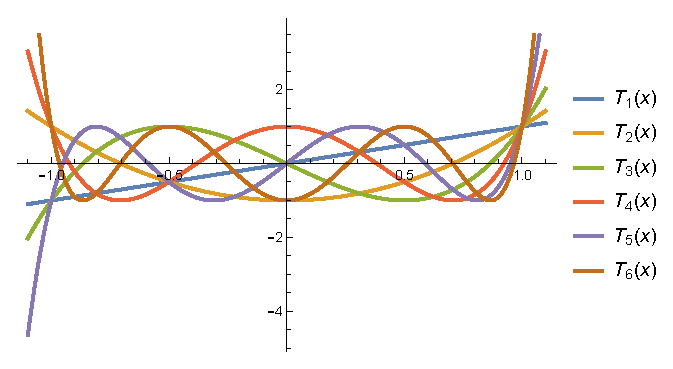
\includegraphics[scale=1.2]{Imagenes/Plot_Polinomios_Chebychev_01.eps}
    \caption{Primeros polinomios de Chebyshev de primera clase.}
    \label{fig:figura_plot_chebychev_01}
\end{figure}
En general, los polinomios de Chebyshev $T_{n}(x)$ satisfacen:
\begin{align*}
T_{n}(-x) = (-1)^{n} \, T_{n} (x)
\end{align*}
que se puede deducir fácilmente a partir de la ec. (\ref{eq:ecuacion_18_056}). También es fácil deducir los siguientes valores especiales:
\begin{align*}
T_{n} (1) &= 1 \\[0.5em]
T_{n} (-1) &= (-1)^{n} \\[0.5em]
T_{2n} (0) &= (-1)^{n} \\[0.5em]
T_{2n+1} (0) &= 0
\end{align*}
Los primeros polinomios de Chebyshev de segunda clase se pueden obtener fácilmente, se presentan a continuación los primeros:
\begin{table}[H]
\centering
\fontsize{14}{14}\selectfont
\begin{tabular}{p{6cm} p{6cm}}
$U_{0}(x) = 1$ & $U_{1} = 2 \, x$ \\[0.5em]
$U_{2}(x) = 4 \, x^{2} - 1$ & $U_{3} = 8 \, x^{3} - 4 \, x$ \\[0.5em]
$U_{4}(x) = 16 \, x^{4} - 12 \, x^{2} + 1$ & $U_{5} = 32 \, x^{5} - 32 \, x^{3} + 6 \, x$ \\[0.5em]
\vdots & \vdots
\end{tabular}
\end{table}
Las funciones que representan a los polinomios de Chebyshev de segunda clase se presentan en la figura (\ref{fig:figura_plot_chebychev_02}):
\begin{figure}[H]
    \centering
    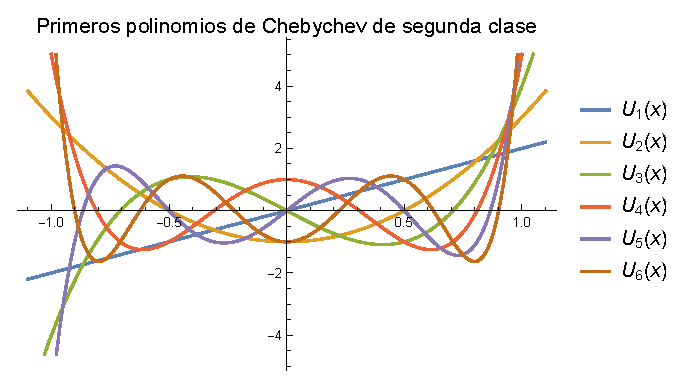
\includegraphics[scale=1.2]{Imagenes/Plot_Polinomios_Chebychev_02.eps}
    \caption{Primeros polinomios de Chebyshev de segunda clase.}
    \label{fig:figura_plot_chebychev_02}
\end{figure}
Los polinomios de Chebyshev $U_{n}(x)$ también satisfacen la propiedad:
\begin{align*}
U_{n} (-x) = (-1)^{n} \, U_{n} (x)
\end{align*}
la cual se puede deducir de las ecs. (\ref{eq:ecuacion_18_057}) y (\ref{eq:ecuacion_18_058}), y tiene, entre otros, los siguientes valores especiales:
\begin{align*}
U_{n} (1) &= n + 1 \\[0.5em]
U_{n} (-1) &= (-1)^{n} \, (n + 1) \\[0.5em]
U_{2n} (0) &= (-1)^{n} \\[0.5em]
U_{2n+1} (0) &= 0
\end{align*}

\newpage
\section{Propiedades de los polinomios de Chebyshev.}

Los polinomios de Chebyshev $T_{n} (x)$ y $U_{n} (x)$ tienen sus principales aplicaciones en el análisis numérico.
\par
Su uso para representar otras funciones en el rango $\abs{x} < 1$ juega un papel importante en la integración numérica; la cuadratura Gauss-Chebyshev es de particular relevancia para la evaluación precisa de integrales cuyos integrandos contienen factores del tipo $(1 - x)^{\pm 1/2}$.
\par
Por tanto, conviene destacar algunas de sus principales propiedades.

\subsection{Fórmula de Rodrigues.}

Los polinomios de Chebyshev $T_{n}(x)$ y $U_{n}(x)$ se pueden expresar en términos de una fórmula de Rodrigues, de manera similar que las otras funciones especiales; se tiene que:
\begin{align*}
T_{n}(x) &= \left[ \dfrac{(-1)^{n} \, \sqrt{\pi} \, (1 - x^{2})^{1/2}}{2^{n} \, \left( n - \dfrac{1}{2} \right)!} \right] \, \dv[n]{x} (1 - x^{2})^{n-1/2} \\[0.5em]
U_{n}(x) &= \left[ \dfrac{(-1)^{n} \, \sqrt{\pi} \, (n+1)}{2^{n+1} \, \left( n - \dfrac{1}{2} \right)! (1 - x^{2})^{1/2}} \right] \, \dv[n]{x} (1 - x^{2})^{n+1/2}
\end{align*}

\subsection{Ortogonalidad mutua.}

La ecuación diferencial de Chebyshev se puede ajustar a una del tipo Sturm-Liouville con $p = (1 - x^{2})^{1/2}$, $\lambda = n^{2}$ y $\rho = (1 - x^{2})^{-1/2}$, su intervalo natural es $[-1, 1]$.
\par
Como los polinomios de Chebyshev de primera clase $T_{n}(x)$, son soluciones de la ecuación diferencial de Chebyshev y son regulares en los puntos extremos $x = \pm 1$, deben de ser mutuamente ortogonales en este intervalo con respecto a la función de peso $\rho = (1 - x^{2})^{1/2}$, es decir:
\begin{align}
\scaleint{6ex}_{\bs -1}^{1} T_{n}(x) \, T_{m}(x) \, (1 - x^{2})^{-1/2} \dd{x} = 0 \hspace{1.5cm} \mbox{si  } n \neq m
\label{ec:ecuacion_18_061}
\end{align}
La ortogonalización cuando $m = n$, es fácil de deducir haciendo la sustitución $x = \cos \theta$ y usando la ec. (\ref{eq:ecuacion_18_055}), de donde se obtiene el resultado:
\begin{align}
\scaleint{6ex}_{\bs -1}^{1} T_{n} (x) \, T_{n} (x) (1 - x^{2})^{-1/2} \dd{x} = \begin{cases}
\pi & \mbox{para  } n = 0 \\[0.5em]
\dfrac{\pi}{2} & \mbox{para  } n = 1, 2, 3, \ldots
\end{cases}
\label{eq:ecuacion_18_062}
\end{align}
Para los polinomios de Chebyshev de segunda clase $U_{n}(x)$, vemos que de la ec. (\ref{eq:ecuacion_18_058}):
\begin{align*}
(1 - x^{2})^{1/2} \, U_{n} (x) = V_{n+1} (x)
\end{align*}
satisface la ecuación diferencial de Chebyshev (\ref{eq:ecuacion_18_054}) con $\nu = n + 1$. Por lo que la relación de ortogonalidad para los $U_{n}(x)$ se obtiene al reemplazar $T_{i}(x)$ por $V_{i+1} (x)$ en la ec. (\ref{ec:ecuacion_18_061}), obteniendo:
\begin{align*}
\scaleint{6ex}_{\bs -1}^{1} U_{n}(x) \, U_{m}(x) \, (1 - x^{2})^{1/2} \dd{x} = 0 \hspace{1.5cm} \mbox{si  } n \neq m
\end{align*}
La correspondiente condición de normalización cuando $n = m$, se puede obtener al hacer nuevamente la sustitución $x  = \cos \theta$:
\begin{align*}
\scaleint{6ex}_{\bs -1}^{1} U_{n}(x) \, U_{n}(x) \, (1 - x^{2})^{1/2} \dd{x} = \dfrac{\pi}{2}
\end{align*}

\subsection{Expansión de funciones.}

Dadas las condiciones de ortogonalización y normalización, permiten que cualquier función (razonable) pueda expandirse en el intervalo $\abs{x} < 1$ en una serie de la forma:
\begin{align*}
f(x) = \dfrac{a_{0}}{2} + \nsum_{n=1}^{\infty} a_{n} \, T_{n} (x)
\end{align*}
en donde los coeficientes en la expresión están dados por:
\begin{align*}
a_{n} = \dfrac{2}{\pi} \scaleint{6ex}_{\bs -1}^{1} f(x) \, T_{n} (x) \, (1 - x^{2})^{-1/2} \dd{x}
\end{align*}
Para los polinomios de Chebyshev de segunda clase, también es posible expandir cualquier función razonable, en el intervalo $\abs{x} < 1$ en una serie de la forma:
\begin{align*}
f(x) = \nsum_{n=0}^{\infty} a_{n} \, U_{n} (x)
\end{align*}
en donde los coeficientes $a_{n}$ están dados por:
\begin{align*}
a_{n} = \dfrac{2}{\pi} \scaleint{6ex}_{\bs -1}^{1} f(x) \, U_{n}(x) \, 
\end{align*}

\subsection{Funciones generatrices.}

Las funciones generatrices para los polinomios de Chebyshev de primera y segunda clase, están dados respectivamente por las expresiones:
\begin{align}
G_{I} (x, h) &= \dfrac{1 - x \, h}{1 - 2 \, x \, h + h^{2}} = \nsum_{n=0}^{\infty} T_{n} (x) \, h^{n} \label{eq:ecuacion_18_063} \\[0.5em]
G_{II} (x, h) &= \dfrac{1}{1 - 2 \, x \, h + h^{2}} = \nsum_{n=0}^{\infty} U_{n} (x) \, h^{n} \label{eq:ecuacion_18_064}
\end{align}
%Estas definiciones pueden probarse de manera similar a la utilizada para la función generadora de los polinomios de Legendre.
Para los polinomios de Chebyshev, las funciones generadoras son de uso menos práctico, ya que la mayoría de los resultados útiles se pueden obtener más fácilmente aprovechando las formas trigonométricas (\ref{eq:ecuacion_18_055}), como se verá a continuación.

\subsection{Relaciones de recurrencia.}

Se cuenta con distintas relaciones de recurrencia útiles para los polinomios de Chebyshev $T_{n}(x)$ y $U_{n}(x)$, la mayoría de ellas se deducen fácilmente al hacer $x = \cos \theta$ y usando las ecs. (\ref{eq:ecuacion_18_055}) y (\ref{eq:ecuacion_18_058}), así tendremos:
\begin{align}
T_{n} (x) &= T_{n} (\cos \theta) = \cos n \theta \label{eq:ecuacion_18_065} \\[0.5em]
U_{n} (x) &= U_{n} (\cos \theta) = \dfrac{\sin (n + 1) \theta}{\sin \theta} \label{eq:ecuacion_18_066} 
\end{align}
Luego, se puede usar la fórmula estándar para las funciones trigonométricas para derivar una amplia variedad de relaciones de recurrencia. De particular utilidad son las identidades trigonométricas:
\begin{align}
\cos (n \pm 1)\theta &= \cos n \theta \, \cos \theta \mp \sin n \theta \, \sin \theta \label{eq:ecuacion_18_067} \\[0.5em]
\sin (n \pm 1)\theta &= \sin n \theta \, \cos \theta \pm \cos n \theta \, \sin \theta \label{eq:ecuacion_18_068}
\end{align}
Dos importantes relaciones de recurrencia son:
\begin{align}
T_{n+1} (x) - 2 \, x \, T_{n} (x) + T_{n-1} (x) &= 0 \label{eq:ecuacion_18_069} \\[0.5em]
U_{n+1} (x) - 2 \, x \, U_{n} (x) + U_{n-1} (x) &= 0 \label{eq:ecuacion_18_070}
\end{align}
Las relaciones de recurrencia (\ref{eq:ecuacion_18_069}) y (\ref{eq:ecuacion_18_070}) son extremadamente útiles en el cálculo práctico de polinomios de Chebyshev. Por ejemplo, dados los valores de $T_{0} (x)$ y $T_{1} (x)$ en algún punto $x$, el resultado dado por la ec. (\ref{eq:ecuacion_18_069}) puede usarse iterativamente para obtener el valor de cualquier $T_{n} (x)$ en ese punto; de manera similar, la ec. (\ref{eq:ecuacion_18_070}) puede usarse para calcular el valor de cualquier $U_{n} (x)$ en algún punto $x$, dados los valores de $U_{0} (x)$ y $U_{1} (x)$ en ese punto.
\par
Otras relaciones de recurrencia que satisfacen los polinomios de Chebyshev son:
\begin{align}
T_{n} (x) &= U_{n}(x) - x \, U_{n-1} (x) \label{eq:ecuacion_18_071} \\[0.5em]
(1 - x^{2}) \, U_{n} (x) &= x \, T_{n+1} (x) - T_{n+2} (x) \label{eq:ecuacion_18_072}
\end{align}
que establecen relaciones útiles entre los dos conjuntos de polinomios $T_{n} (x)$ y $U_{n} (x)$. La relación (\ref{eq:ecuacion_18_071}) se sigue inmediatamente de (\ref{eq:ecuacion_18_068}), mientras que la ec. (\ref{eq:ecuacion_18_072}) se sigue de la ec. (\ref{eq:ecuacion_18_067}), con $n$ reemplazado por $n + 1$, al observar que $\sin \theta = 1 - x^{2}$. Pueden obtenerse resultados útiles adicionales relacionados con los derivadas de los polinomios de Chebyshev a partir de las ecs. (\ref{eq:ecuacion_18_065}) y (\ref{eq:ecuacion_18_066}):
\begin{align*}
\pderivada{T}_{n} (x) &= n \, U_{n-1} (x) \\[0.5em]
(1 - x^{2}) \, \pderivada{U}_{n} (x) &= x \, U_{n} (x) - (n + 1) \, T_{n+1} (x)
\end{align*}

\section{Minimizando el error de interpolación.}

\subsection{Interpolación de puntos.}

Un polinomio de interpolación es un polinomio que pasa exactamente a través de un conjunto dado de puntos.
\par
Ajuste por interpolación:
\begin{figure}[H]
   \centering
   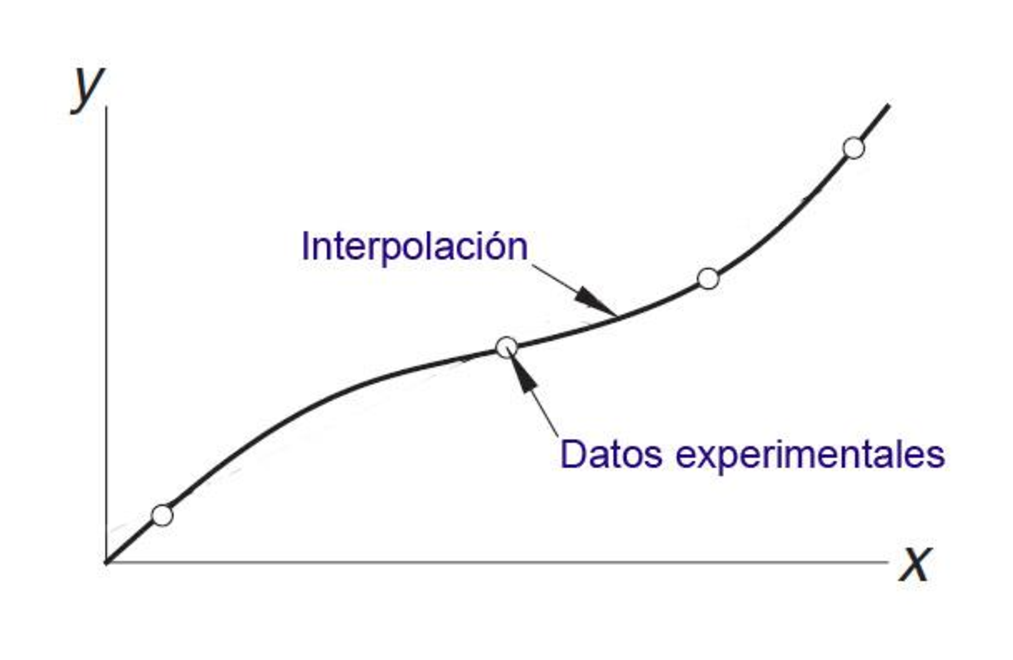
\includegraphics[scale=0.5]{Imagenes/Interpol02.eps}
   \caption{En la interpolación, la curva toca los datos experimentales.}
\end{figure}

Ajuste de la curva:
\begin{figure}[H]
   \centering
   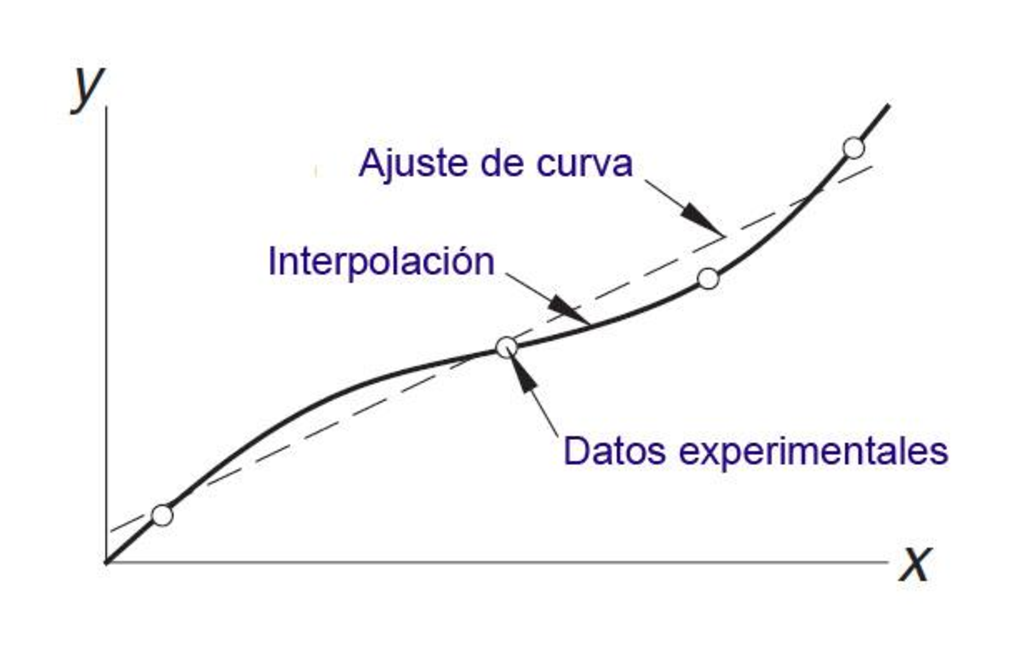
\includegraphics[scale=0.5]{Imagenes/Interpol03.eps}
   \caption{Mientras que al ajustar una curva, se busca una curva con expresión conocida intentando minimizar la diferencia entre la curva original y la aproximación.}
\end{figure}

Supongamos que lo que se quiere es buscar un polinomio de grado finito que aproxime una función dada. Lo que resulta intuitivo es buscar que dicho polinomio tenga el mismo valor de la función en un conjunto de puntos dado.
\par
Sabiendo que por $n$ puntos pasa un único polinomio de grado $n-1$, podríamos argumentar que la única manera de buscar una aproximación mejor del polinomio a la función es la de escoger de formas distintas los puntos por los cuales el polinomio ha de pasar.
\par
Dada una función $f(x)$ de la cual se conocen sus valores en un número finito de puntos $x_{0}, x_{1}, \ldots, x_{m}$, se llama \emph{interpolación polinómica} al proceso de hallar un polinomio $p_{m}(x)$ de grado menor o igual a $m$, cumpliendo $p_{m}(x_{k}) = f(x_{k})$ parar cada $k = 1, 2, \ldots, m$.
\par
Los coeficientes $a_{0}, a_{1}, a_{2}, \ldots, a_{n}$, de dicho polinomio se obtienen imponiendo al polinomio de pasar por los puntos fijados.
\begin{align*}
\mqty[
x_{0}^{n} & x_{0}^{n-1} & x_{0}^{n-2} & \ldots & x_{0} & 1 \\
x_{1}^{n} & x_{1}^{n-1} & x_{1}^{n-2} & \ldots & x_{1} & 1 \\
\vdots & \vdots & \vdots & & \vdots & \vdots \\
x_{n}^{n} & x_{n}^{n-1} & x_{n}^{n-2} & \ldots & x_{n} & 1 
]
\mqty[
a_{n} \\ a_{n-1} \\ \vdots \\ a_{0}
]
=
\mqty[
y_{0} \\ y_{1} \\ \vdots \\ y_{n}
]
\end{align*}

Este sistema es compatible y a la matriz asociada se le suele denominar \emph{matriz de Vandermonde}. La complejidad computacional para invertir la matriz es de $\order{n^{3}}$.
\par
Por esta razón, han sido construidos diferentes algoritmos que aprovechan la particular estructura de este sistema que reducen la complejidad a $\order{n^{2}}$, como el \emph{método de Lagrange} o el \emph{método de las diferencias divididas de Newton}.

\subsection{Interpolación de Lagrange.}

El polinomio interpolador de grado $n$ de Lagrange es un polinomio de la forma:
\begin{align*}
p_{n}(x) = \nsum_{j=0}^{k} f_{j}(x) \, l_{j}(x) \hspace{1.5cm} n \leq m
\end{align*}
Donde los $l_{j}(x)$ son los llamados \emph{polinomios de Lagrange}, que se calculan como:
\begin{align*}
&{}l_{j}(x) = \prod_{j \neq i} \dfrac{x - x_{i}}{x_{j} - x_{i}} \\[0.5em]
&= \dfrac{(x - x_{0})(x - x_{i}) \ldots(x - x_{j-1})(x - x_{j+1}) \ldots (x - x_{n})}{(x_{j} - x_{0})(x_{j} - x_{1}) \ldots(x_{j} - x_{j-1})(x_{j} - x_{j+1}) \ldots (x_{j} - x_{n})}
\end{align*}

Por ejemplo: se quiere hallar el valor de la función:
\begin{align*}
f(x) = e^{x+1}
\end{align*}
Utilizando un polinomio de interpolación de Lagrange de grado $2$ que pase por los puntos:
\begin{table}[H]
\centering
\large
\begin{tabular}{c | c}
$x$ & $f(x)$ \\ \hline
$0$ & $f(0)$ \\
$0.5$ & $f(0.5)$ \\
$1$ & $f(1)$ \\
\end{tabular}
\end{table}

Al graficar los puntos tendremos lo siguiente:
\begin{figure}[H]
   \centering  
   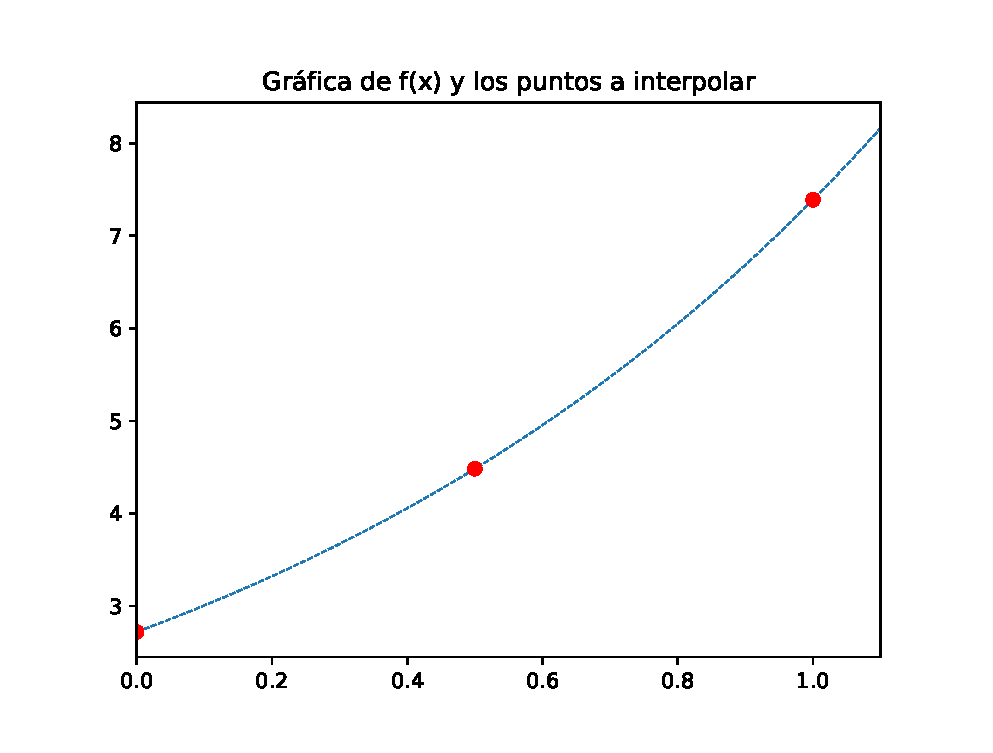
\includegraphics[scale=0.65]{Imagenes/Ejemplo_interpolacion_Chebychev_01.eps}
\end{figure}

Usamos el método directo para calcular el polinomio de interpolación. Con las condiciones dadas, los polinomios de Lagrange son:
\begin{align*}
l_{0} (x) &= \dfrac{(x - 0.5)(x - 1)}{0.5} = 2 \, x^{2} - 3 \, x + 1 \\[0.5em]
l_{1} (x) &= \dfrac{x (x - 1)}{-0.25} = - 4 \, x^{2} + 4 \, x \\[0.5em]
l_{2} (x) &= \dfrac{x (x - 0.5)}{0.5} = 2 \, x^{2} - x
\end{align*}

El polinomio de interpolación de Lagrange de grado $2$ es:
\begin{align*}
p_{2}(x) &= \nsum_{j=0}^{2} f_{j}(x) \, l_{j}(x) = \\[0.5em]
&= (2 \, e - 4 \, e^{3/2} + 2 \, e^{2}) \, x^{2} + \\[0.5em]
&+ (-3 \, - 4 \, e^{3/2} + 2 \, e^{2}) \, x + e
\end{align*}

Una pregunta que puede surgir al utilizar un polinomio de interpolación para aproximar una función es qué tan bueno es el ajuste del polinomio a la función originaria.
\par
Por esta razón consideramos el error de interpolación de un polinomio de grado $n$ que pase por los puntos de una función $f(x)$ en los puntos $x_{0}, \ldots, x_{n}$.
\par
Si $f(x)$ es una función determinada en $x_{0}, \ldots, x_{n}$ y es $n$ veces diferenciable, entonces el \emph{error de interpolación} puede calcularse como valor absoluto de la diferencia entre la función y el polinomio.
\par
Construimos una función $\phi(x)$ por la cual se cumpla que
\begin{align*}
&\phi(x) = f(x) {-} p_{n}(x) {-} a(x)(x {-} a_{0})(x {-} a_{1}) \ldots (x {-} a_{n}) \\[0.5em]
&\exists \, \bar{x} \in [-1, 1] \\[0.5em]
&a(\bar{x}) = \big[ f(x) {-} p_{n} \big] (x {-} a_{0})(x {-} a_{1}) \ldots (x {-} a_{n}) = 0
\end{align*}

Esta función se anula en $n + 2$ puntos. Aplicando el \emph{teorema de Rolle} se tiene que una función que toma el mismo valor $n + 2$ veces tiene $n + 1$ puntos que anulan la derivada. A la vez, la derivada de esta función es tal que, teniendo $n + 1$ puntos con el mismo valor tendrá $n$ puntos que anulan su derivada. 
\par
Por lo tanto, derivando sucesivamente $n + 1$ veces, tenemos que existirá un único punto $\zeta$ que anule la derivada $n+1$-ésima, es decir:
\begin{align*}
\phi^{n+1} \, (\zeta) = 0
\end{align*}
Así podemos asegurar que $\phi^{n+1}$ tiene al menos una raíz, con lo cual resulta evidente que, siendo $p_{n}(x)$ un polinomio de grado mayor que $n - 1$, $\phi^{n+1} \, (\zeta)$ resultará la siguiente:
\begin{align*}
\phi^{n+1} \, (x) = f^{(n+1)} \, (\bar{x}) - a (\bar{x}) (n + 1)!
\end{align*}

Por consiguiente, al haber dejado que en $\phi^{n+1} \, (\bar{x}) = 0$, se tiene que:
\begin{align*}
a (\bar{x}) = \dfrac{f^{(n+1)} \, (\bar{x})}{(n + 1)!}
\end{align*}
En el caso de que $f(x)$ sea $n$ veces diferenciable en el dominio $[-1, 1]$, el error de interpolación podrá definirse como:
\begin{align*}
f(x) - p_{n}(x) = \dfrac{f^{(n+1)}(\xi)}{(n + 1)!} \, \prod_{i} (x - x_{i})
\end{align*}
Donde $\xi$ es un punto que pertenece a $[-1, 1]$, por lo cual $\phi^{(n+1)}(\zeta) = 0$.
\par
Adjudicando valores absolutos en la expresión del error de interpolación y maximizando ambos lados de la desigualdad a lo largo del intervalo $[-1, 1]$ obtenemos la cota para dicho error:
\begin{align*}
&\max_{\abs{x} < 1} \abs{f(x) - p_{n}(x)} = \abs{\dfrac{f^{(n+1)}(\xi)}{(n + 1)!} \, \prod_{i} (x - x_{i})} \leq \\[0.5em]
&\leq \dfrac{\displaystyle \max_{\abs{x} < 1} \abs{f^{(n+1)}(\xi)}}{(n+1)!} \, \max_{\abs{x} < 1} \prod_{i} (x - x_{i})
\end{align*}

Dada la unicidad del polinomio de interpolación, las únicas dos cosas que podemos mover a la hora de reducir el error de interpolación es el grado del polinomio (por consiguiente, el número de puntos) y la localización de dichos puntos. Se podría creer que al aumentar el grado del polinomio el error de interpolación se reduzca. 
\par
En realidad, pese al ser un resultado antiintuitivo, Carle David Tolmé Runge observó que el error de interpolación en un intervalo dado, tiende a infinito cuando el grado del polinomio de interpolación tiende a infinito. Es decir:
\begin{align*}
\lim_{n \to \infty} \big( \max_{\abs{x} < 1} \abs{f(x) - p_{n}(x)} \big) = \infty
\end{align*}

El método que veremos nos permite proporcionar los puntos por los cuales hacer pasar el polinomio de interpolación de forma tal que la distancia máxima entre el polinomio interpolado y la función originaria sea mínima.
\par
La oscilación observada por Runge se puede minimizar usando nodos de Chebyshev en lugar de nodos equidistantes En este caso se garantiza que el error máximo disminuye al crecer el orden polinómico.

\subsection{Las raíces de los polinomios de Chebyshev.}

Esta es una propiedad que hace particularmente interesante el utilizar las raíces de los polinomios de Chebyshev como puntos por donde interpolar el polinomio.
\par
Para minimizar el último factor de la cota del error, Pafnuty Lvovich Chebyshev demostró que los puntos $x_{0}, \ldots, x_{n}$ por los cuales hacer pasar el polinomio, han de ser escogidos de forma que:
\begin{align*}
\max_{\abs{x} < 1} \prod_{i} (x - x_{i}) = \dfrac{1}{2^{n}} \, T_{n+1} (x)
\end{align*}
donde $T_{n+1}(x)$ es el polinomio de Chebyshev de primera clase de orden $n + 1$.
\par
Entre todas las elecciones de los puntos $x_{0}, \ldots, x_{n}$, elegirlos de forma que la siguiente expresión se respete:
\begin{align*}
\phi^{n+1} \, (x) = f^{(n+1)} \, (\bar{x}) - a (\bar{x}) (n + 1)!
\end{align*}
Se garantiza que el polinomio así obtenido es el polinomio único que tenga la propiedad:
\begin{align*}
\max_{\abs{x} < 1} T_{n} (x) &\leq \max_{\abs{x} < 1} \prod (x - x_{i}) \\[0.5em]
\max_{\abs{x} < 1} T_{n} (x) &= \dfrac{1}{2^{n}} \\[0.5em]
\dfrac{1}{2^{n}} &\leq \max_{\abs{x} < 1} T_{n} (x)
\end{align*}

Se puede demostrar que el valor absoluto de la diferencia entre la función y el polinomio interpolado por las raíces del polinomio de Chebyshev resulta acotado de la siguiente forma:
\begin{align*}
\abs{f(x) - p_{n-1}} \leq \dfrac{1}{2^{n-1} \, n!} \, \max_{\xi \in [-1, 1]}  \, \abs{f^{n} \, (\xi)}
\end{align*}

\subsection{Interpretación geométrica.}

Una interpretación geométrica de las raíces de Chebyshev es aquella según la cual estos se colocan en un segmento de longitud igual al diámetro de un círculo, cuya circunferencia repartimos en $n$ partes iguales.
\par
Proyectando a lo largo del dicho segmento el punto medio de cada partición de la semicircunferencia obtenemos puntos que coinciden con las raíces del polinomio de Chebyshev.
\begin{figure}[H]
    \centering
    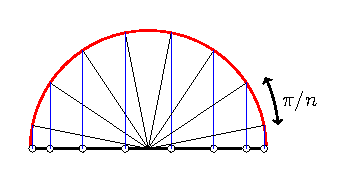
\includegraphics[scale=1]{Imagenes/Nodos_Chebychev_01.eps}
\end{figure}

La razón por la cual la aproximación de una función $f(x)$ por un polinomio que interpole puntos escogidos de esta forma minimiza el efecto Runge es que la densidad de puntos resulta creciente desde el centro hasta los extremos.
\par
Para calcular dichas raíces utiliza la identidad trigonométrica del polinomio de Chebyshev:

La razón por la cual la aproximación de una función $f(x)$ por un polinomio que interpole puntos escogidos de esta forma minimiza el efecto Runge es que la densidad de puntos resulta creciente desde el centro hasta las extremidades.
\par
Para calcular dichas raíces utiliza la identidad trigonométrica del polinomio de Chebyshev:
\begin{align*}
T_{n}(x) = \cos (n \, \arccos x) = \cosh (n \, \mbox{arccosh} \, x)
\end{align*}
Este coseno se anula cuando la expresión al interior es un múltiplo de $2 \, \pi$.  Por lo tanto las raíces del polinomio de Chebyshev en $[-1,1]$ son:
\begin{align*}
x_{i} = \cos \left( \dfrac{2 \, i - 1}{2 \, n} \, \pi \right) \hspace{1cm} i = 1, 2, \ldots, n
\end{align*}

En el caso de que se quisiera definir el polinomio de Chebyshev en un intervalo cualquiera $[a, b]$, las raíces se trasforman como:
\begin{align*}
x_{i} = \dfrac{a + b}{2} &+ \dfrac{b - a}{2} \, \cos \left( \dfrac{2 \, i - 1}{2 \, n} \, \pi \right) \\[0.5em] 
i =& 0, 1, \ldots, n
\end{align*}

La utilización de los nodos de Chebyshev nos permite también utilizar un método recursivo para la obtención de los coeficientes:
\begin{align*}
f(x) \simeq \nsum_{j=0}^{n} c_{j} \, T_{j}(x)
\end{align*}
donde los coeficientes $c_{j}$ son:
\begin{align*}
c_{0} &= \dfrac{1}{n + 1} \, \nsum_{j=0}^{n} f(x_{k}) \, T_{0}(x_{k}) = \dfrac{1}{n + 1} \, \nsum_{j=0}^{n} f(x_{k}) \\[0.5em]
c_{j} &= \dfrac{1}{n + 1} \, \nsum_{j=0}^{n} f(x_{k}) \, T_{j}(x_{k})
\end{align*}
Esta fórmula permita calcular los coeficientes del polinomio de interpolación con un costo computacional del orden de $\order{n^{2}}$ operaciones.

\subsection{Ejercicio con las raíces de los \texorpdfstring{$T_{n}(x)$}{Tn(x)}.}

Consideramos la función:
\begin{align*}
f(x) = \dfrac{800 \, x}{54 \, x^{4} + x^{2} + 3}
\end{align*}
para interpolar dos polinomios de igual grado a los puntos de dicha función, en el intervalo $[-1, 1]$.
\par
La función a interpolar es la siguiente:
\begin{figure}[H]
    \centering
    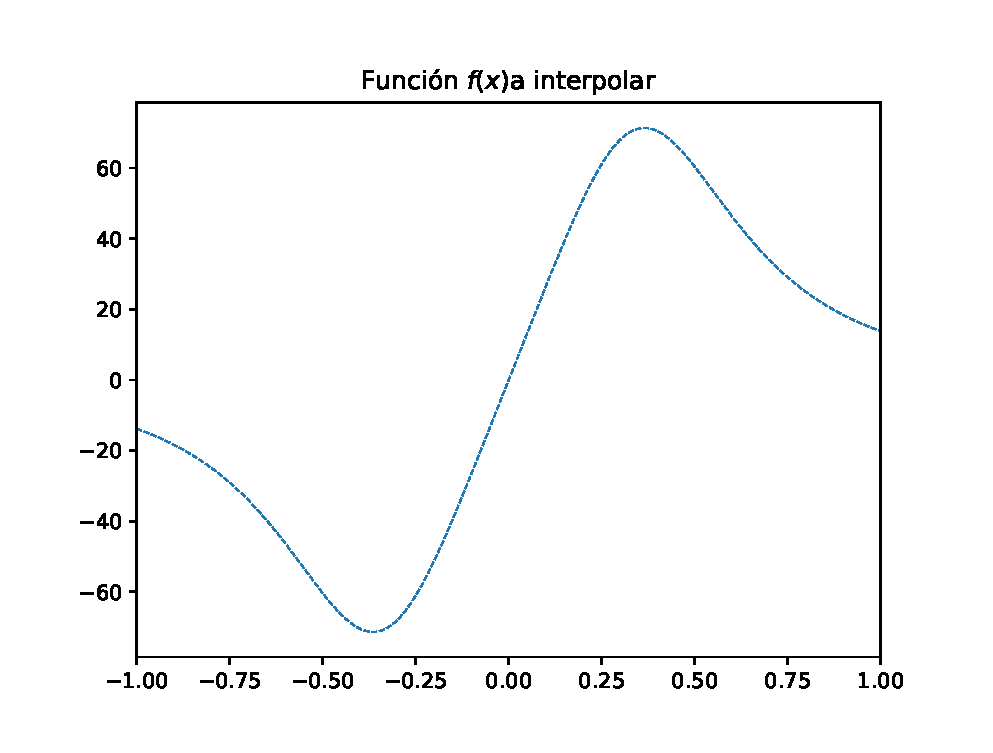
\includegraphics[scale=0.75]{Imagenes/Plot_Ejercicio_Chebychev_01.eps}
\end{figure}

El primer polinomio lo interpolamos con puntos equidistantes y el segundo en las raíces del polinomio de Chebyshev. Utilizamos dos medidas de distancia para evaluar la bondad de la aproximación.

El error debido a la diferencia del área al cuadrado entre la función y el polinomio de interpolación:
\begin{align*}
d_{1} (f, p) = \scaleint{6ex}_{\bs a}^{b} \big[ f(x) - p(x) \big]^{2} \dd{x}
\end{align*}

La segunda medida para medir la bondad de la aproximación es la distancia máxima entre los puntos entre la función y el polinomio de interpolación:
\begin{align*}
d_{2} (f, p) = \max_{x} \abs{f(x) - p(x)}
\end{align*}

\subsection{Implementación con python.}

Con la finalidad de ocupar un lenguaje más versátil para resolver el ejercicio, usamos el lenguaje de programación \texttt{python} y las librerías\footnote{La sintaxis de programación de \texttt{python} no es complicada, pero requiere un manejo preciso en las instrucciones, la notación \texttt{módulo.librería.función} es la que se ocupa, por ello se indican de esta manera las funciones en el listado.} con las cuales podremos obtener los valores de $d_{1}$ y $d_{2}$, así como las gráficas de los procesos de aproximación con los puntos equidistantes y con los puntos de las raíces de los polinomios de Chebyshev.
\par
Se ocuparán las siguientes librerías:
\begin{enumerate}[label=\alph*)]
\item \texttt{numpy.polyfit}
\item \texttt{numpy.poly1d}.
\item \texttt{scipy.integrate.quad}
\item \texttt{scipy.special.roots\_chebyt}
\item \texttt{matplotlib.pyplot}
\end{enumerate}

Se calculan los valores de las $d_{1}$, $d_{2}$, así como las gráficas del ajuste polinomial con puntos equidistantes y con las raíces del polinomio de Chebyshev para el conjunto de puntos:
\begin{align*}
n = 3, 5, 8, 10, 12, 14, 16
\end{align*}
que se presentan a continuación:

\newpage

Con $n = 3$:
\\
\begin{minipage}{0.45\linewidth}
    \begin{figure}[H]
    \centering
    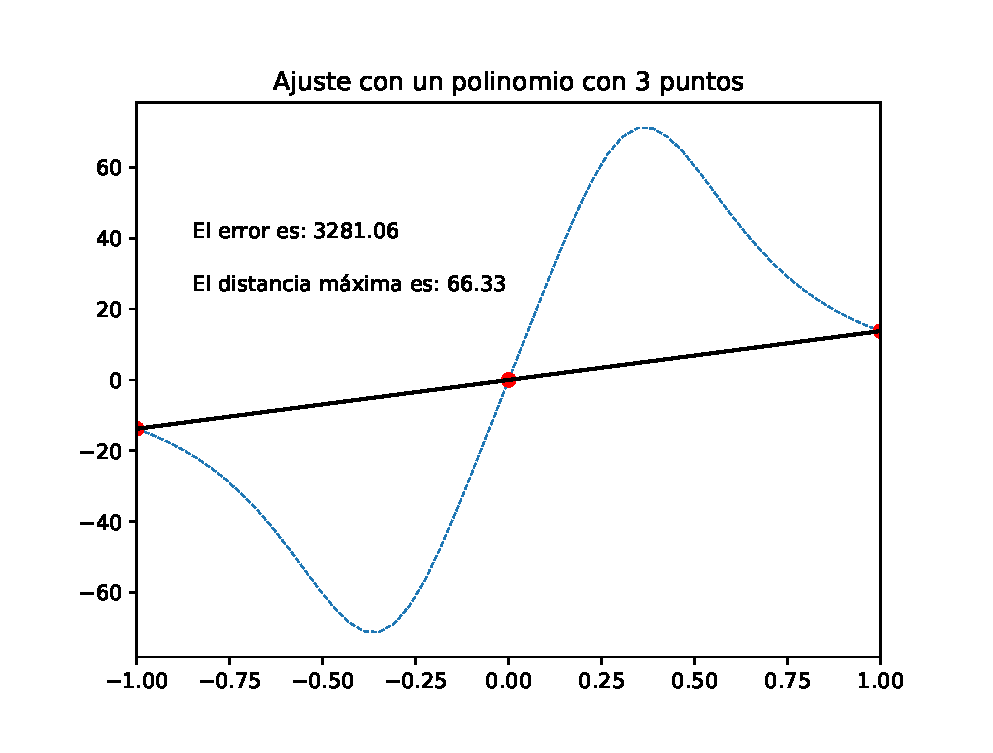
\includegraphics[scale=0.44]{Imagenes/Interpolacion_Chebychev_03_Polinomio.eps}
\end{figure}       
\end{minipage}
\hspace{0.1cm}
\begin{minipage}{0.45\linewidth}
\begin{figure}[H]
    \centering
    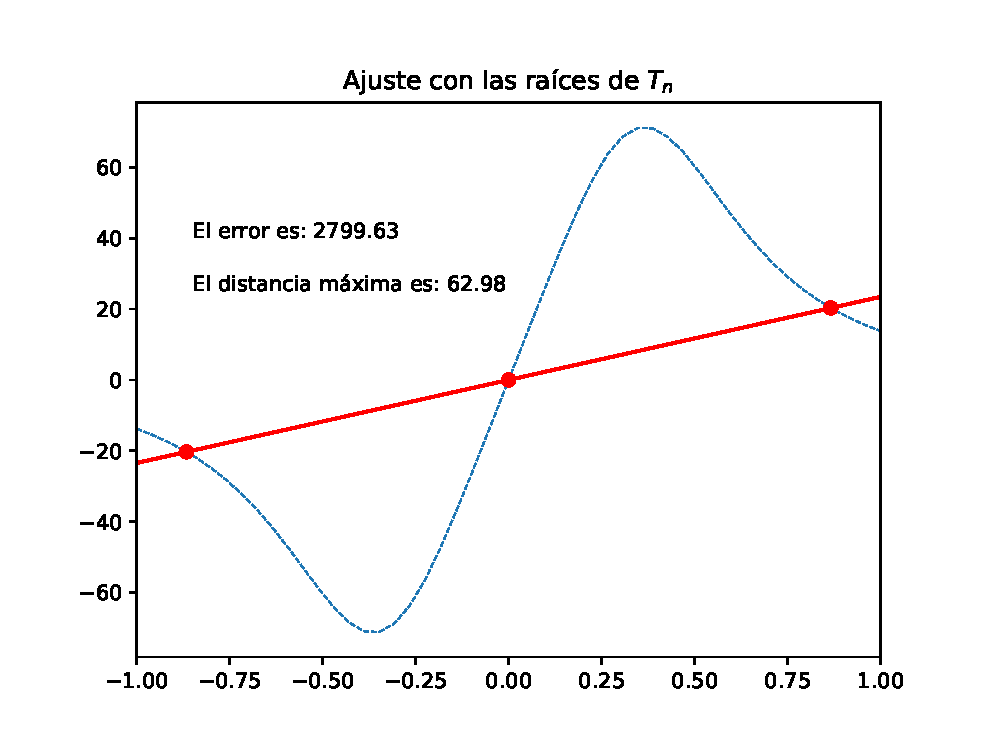
\includegraphics[scale=0.44]{Imagenes/Interpolacion_Chebychev_03_Raices.eps}
\end{figure}
\end{minipage}

Con $n = 5$:
\\
\begin{minipage}{0.45\linewidth}
    \begin{figure}[H]
    \centering
    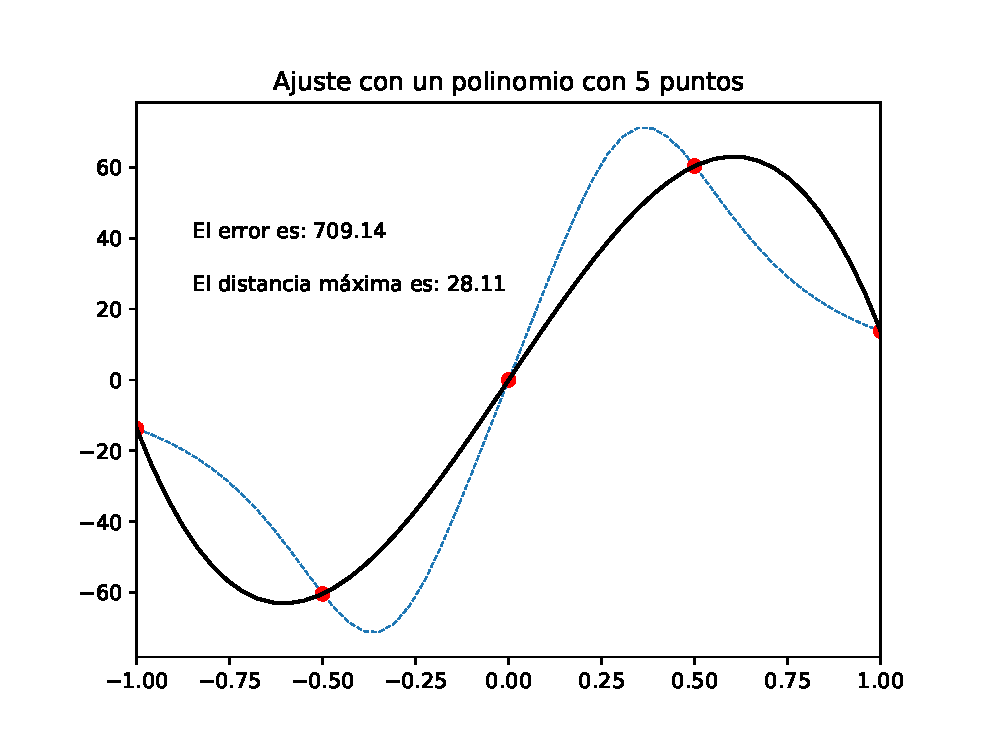
\includegraphics[scale=0.44]{Imagenes/Interpolacion_Chebychev_05_Polinomio.eps}
    \end{figure}       
\end{minipage}
\hspace{0.1cm}
\begin{minipage}{0.45\linewidth}
\begin{figure}[H]
    \centering
    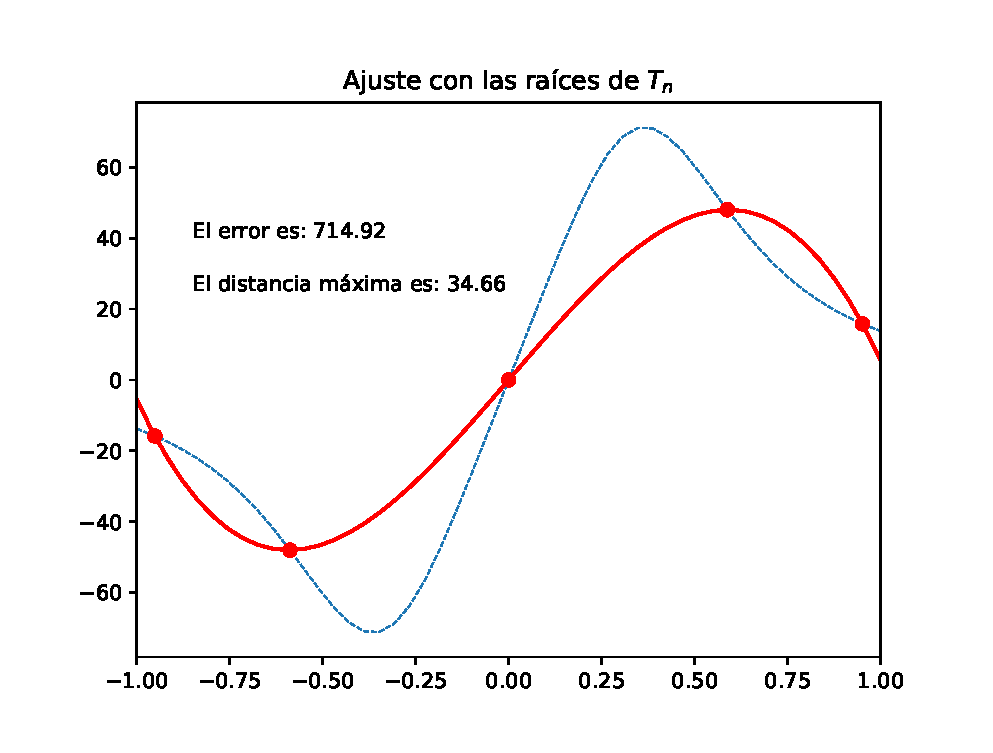
\includegraphics[scale=0.44]{Imagenes/Interpolacion_Chebychev_05_Raices.eps}
\end{figure}
\end{minipage}

Con $n = 8$
\\
\begin{minipage}{0.45\linewidth}
    \begin{figure}[H]
    \centering
    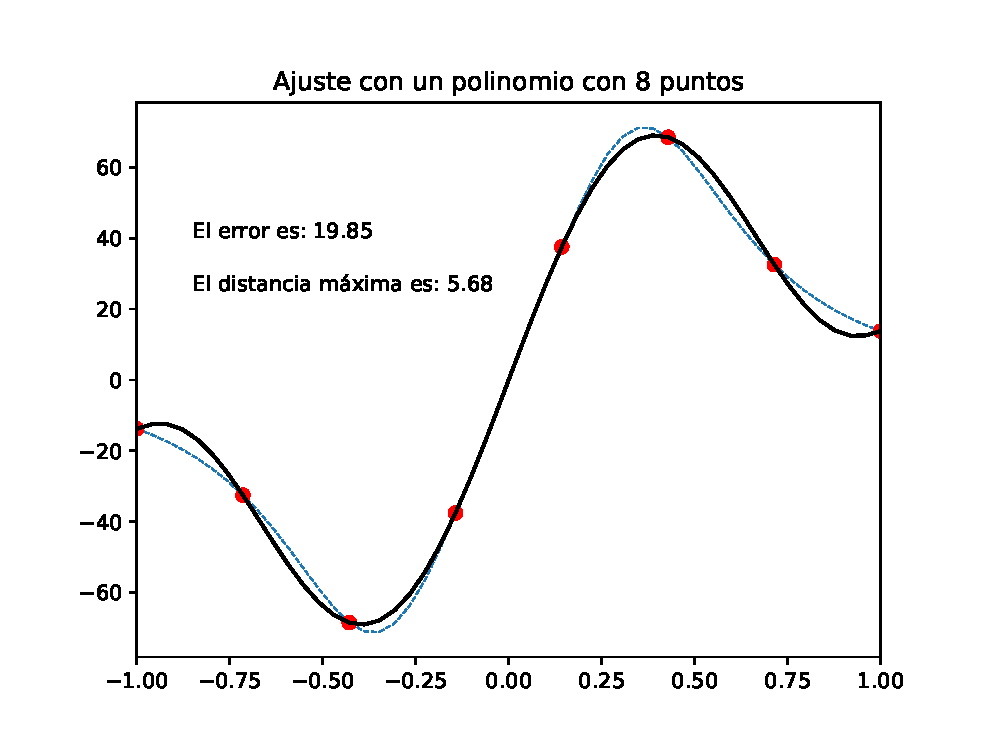
\includegraphics[scale=0.44]{Imagenes/Interpolacion_Chebychev_08_Polinomio.eps}
    \end{figure}       
\end{minipage}
\hspace{0.1cm}
\begin{minipage}{0.45\linewidth}
\begin{figure}[H]
    \centering
    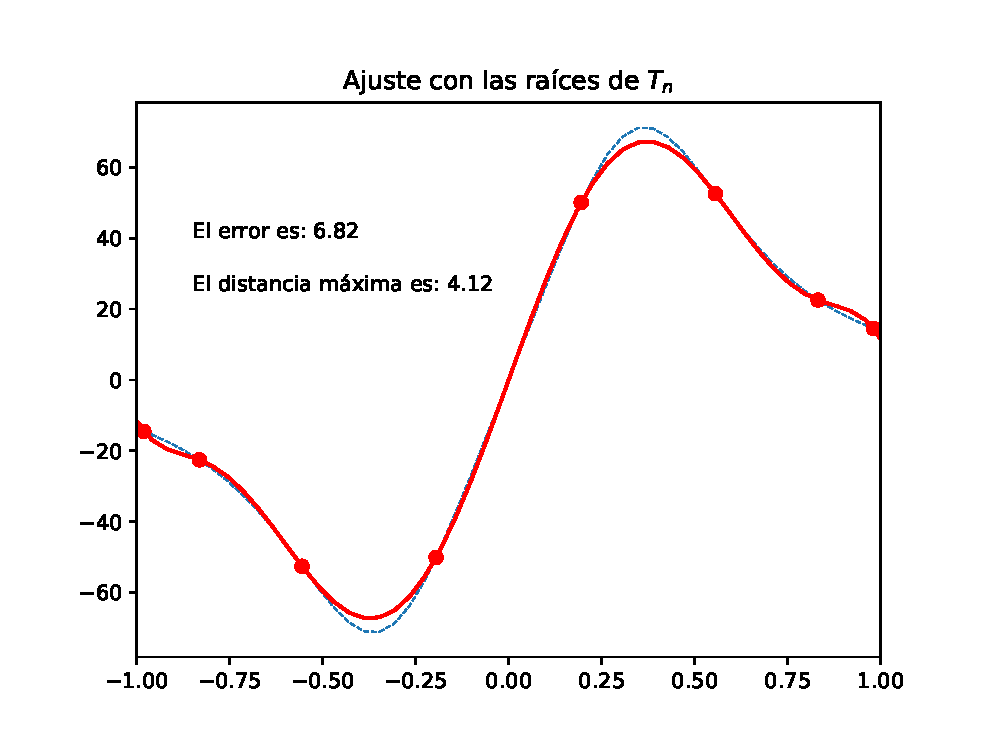
\includegraphics[scale=0.44]{Imagenes/Interpolacion_Chebychev_08_Raices.eps}
\end{figure}
\end{minipage}

\newpage
Con $n = 10$
\\
\begin{minipage}{0.45\linewidth}
    \begin{figure}[H]
    \centering
    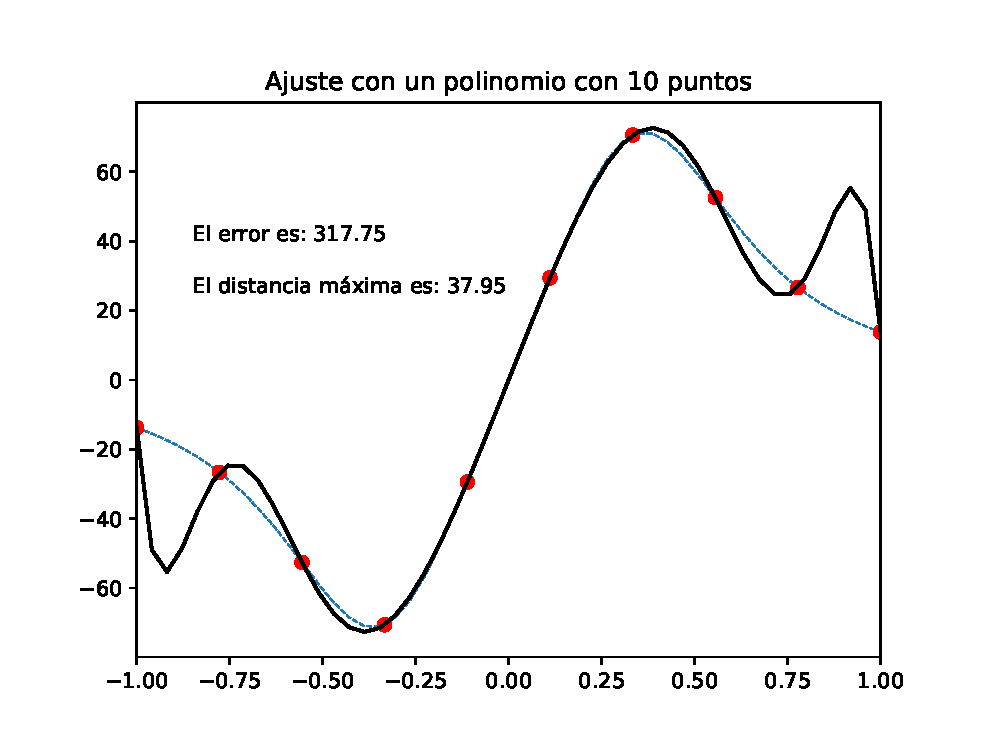
\includegraphics[scale=0.44]{Imagenes/Interpolacion_Chebychev_10_Polinomio.eps}
    \end{figure}       
\end{minipage}
\hspace{0.1cm}
\begin{minipage}{0.45\linewidth}
\begin{figure}[H]
    \centering
    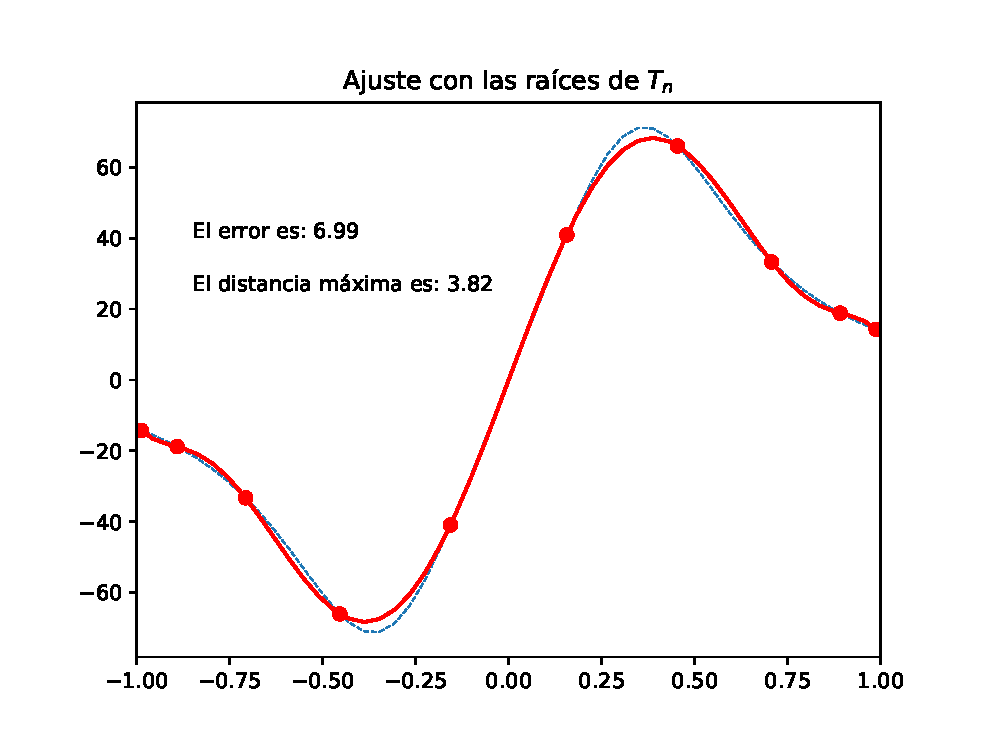
\includegraphics[scale=0.44]{Imagenes/Interpolacion_Chebychev_10_Raices.eps}
\end{figure}
\end{minipage}

Con $n = 12$
\\
\begin{minipage}{0.45\linewidth}
    \begin{figure}[H]
    \centering
    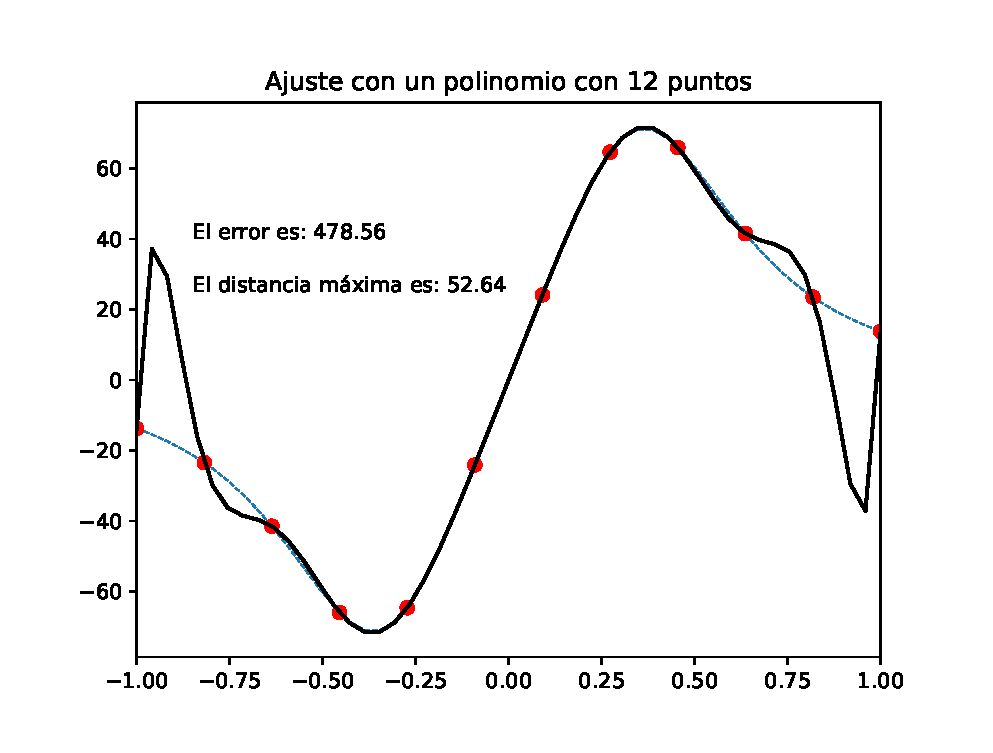
\includegraphics[scale=0.44]{Imagenes/Interpolacion_Chebychev_12_Polinomio.eps}
    \end{figure}       
\end{minipage}
\hspace{0.1cm}
\begin{minipage}{0.45\linewidth}
\begin{figure}[H]
    \centering
    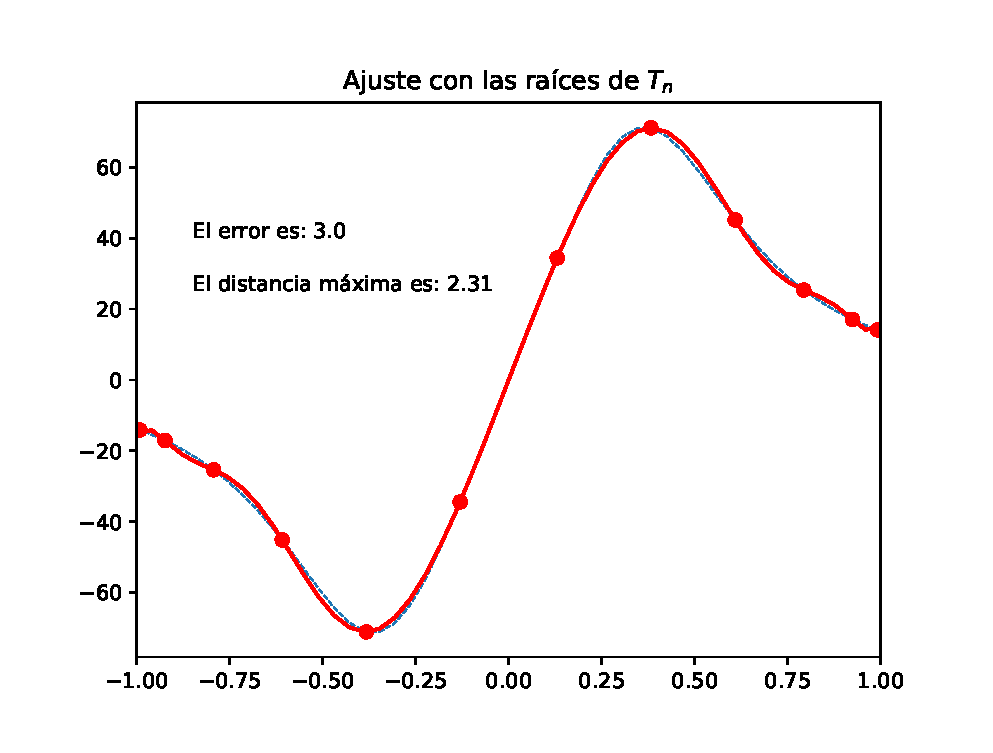
\includegraphics[scale=0.44]{Imagenes/Interpolacion_Chebychev_12_Raices.eps}
\end{figure}
\end{minipage}

Con $n = 14$
\\
\begin{minipage}{0.45\linewidth}
    \begin{figure}[H]
    \centering
    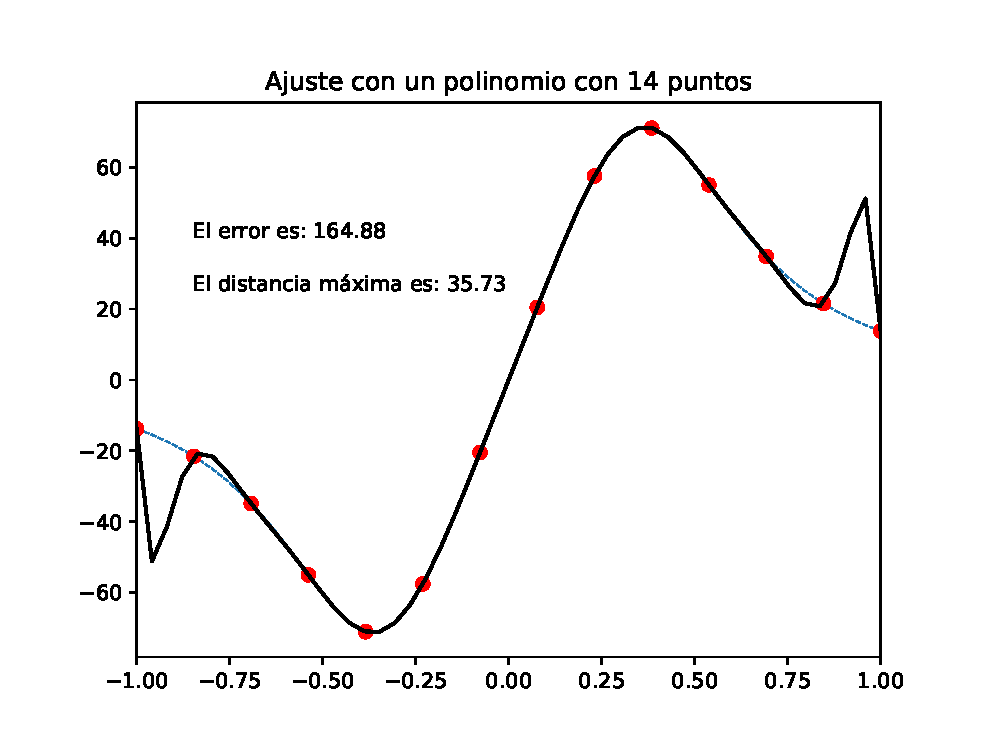
\includegraphics[scale=0.44]{Imagenes/Interpolacion_Chebychev_14_Polinomio.eps}
    \end{figure}       
\end{minipage}
\hspace{0.1cm}
\begin{minipage}{0.45\linewidth}
\begin{figure}[H]
    \centering
    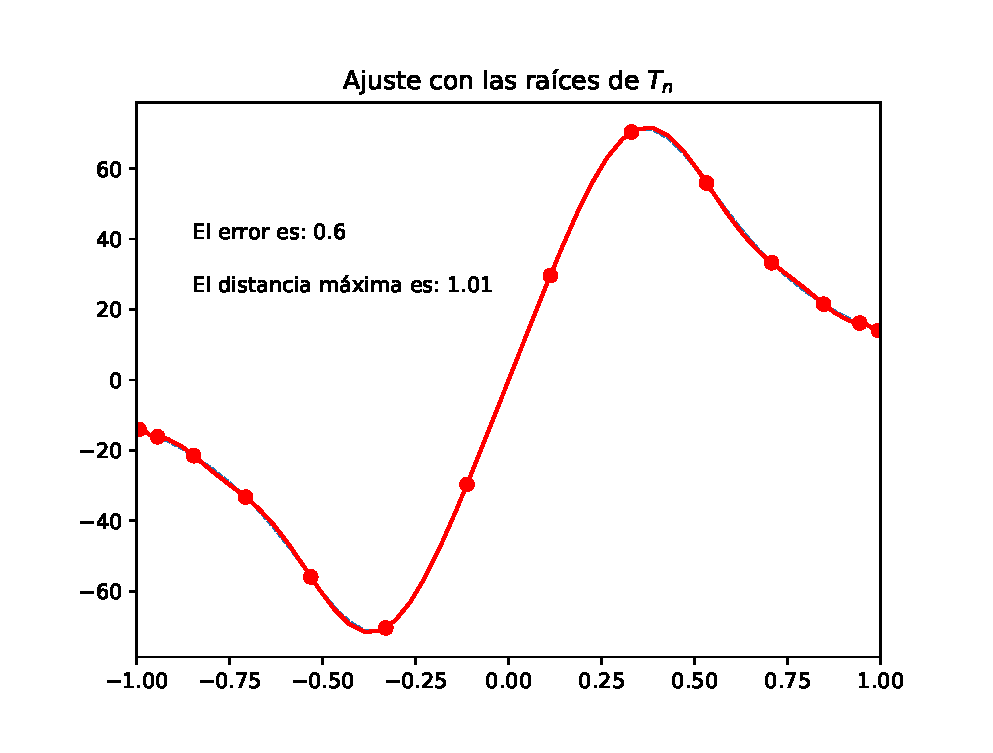
\includegraphics[scale=0.44]{Imagenes/Interpolacion_Chebychev_14_Raices.eps}
\end{figure}
\end{minipage}

\newpage

Con $n = 16$:
\\
\begin{minipage}{0.45\linewidth}
    \begin{figure}[H]
    \centering
    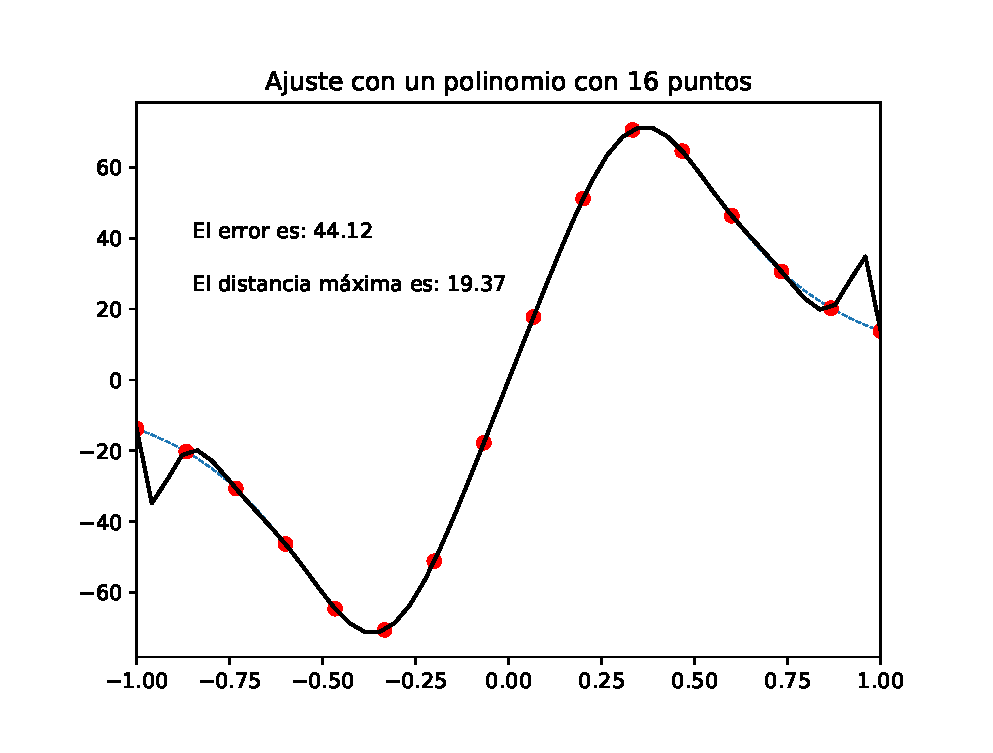
\includegraphics[scale=0.44]{Imagenes/Interpolacion_Chebychev_16_Polinomio.eps}
    \end{figure}       
\end{minipage}
\hspace{0.1cm}
\begin{minipage}{0.45\linewidth}
\begin{figure}[H]
    \centering
    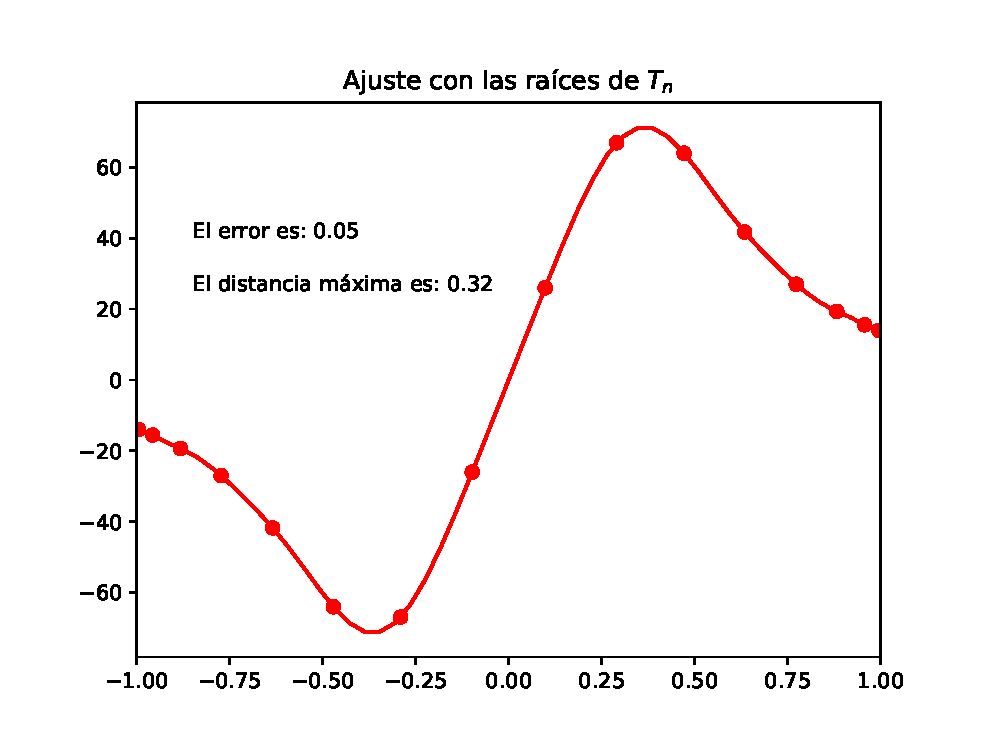
\includegraphics[scale=0.44]{Imagenes/Interpolacion_Chebychev_16_Raices.eps}
\end{figure}
\end{minipage}
\vspace*{0.5em}
\begin{wraptable}{r}{0.4\linewidth}
\caption{Resultados con los métodos de interpolación y del uso de las raíces de los $T_{n}(x)$.}\label{tab:tabla_01}
\begin{tabular}{| c | c | c |} \hline
puntos & $d_{1}$ & $d_{2}$ \\\hline
\multirow{2}{*}{$3$} & $3281.06$ & $66.33$ \\ \cline{2-3}
 & $2799.63$ & $62.98$ \\ \hline
\multirow{2}{*}{$5$} & $709.14$ & $28.11$ \\ \cline{2-3}
 & $714.92$ & $34.66$ \\ \hline 
\multirow{2}{*}{$8$} & $19.85$ & $5.68$ \\ \cline{2-3}
 & $6.82$ & $4.12$ \\ \hline
\multirow{2}{*}{$10$} & $317.75$ & $37.95$ \\ \cline{2-3}
 & $6.99$ & $3.82$ \\ \hline
\multirow{2}{*}{$12$} & $478.56$ & $52.64$ \\ \cline{2-3}
 & $3.0$ & $2.31$ \\ \hline 
\multirow{2}{*}{$14$} & $164.88$ & $35.73$ \\ \cline{2-3}
 & $0.6$ & $1.01$ \\ \hline
\multirow{2}{*}{$16$} & $44.12$ & $19.73$ \\ \cline{2-3}
 & $0.05$ & $0.32$ \\ \hline
\end{tabular}
\end{wraptable}

\textbf{Conclusión: } Lo que encontramos claramente es que el método con las raíces del polinomio de Chebyshev resulta óptimo para la minimización de la mayor distancia existente entre la función que se desea aproximar $f(x)$ y el polinomio que se construye con las raíces de Chebyshev (ver la Tabla \ref{tab:tabla_01}).
\par
Sin embargo, esto no garantiza de ninguna forma la minimización del otras distancias, como se observó en caso de la norma $d_{1}$.
\par
Un inconveniente considerable de dicho método es que si queremos añadir más puntos, se tendría que estimar de nuevo los coeficientes de los polinomios de Chebyshev.
\par
Con un algoritmo en \texttt{python}, se simplifica esta tarea ya que el cálculo se realiza nuevamente al modificar el número de puntos $n$, las demás tareas ya quedan establecidas en funciones que se mandan llamar.

% \section{Ejercicios a cuenta.}

% %ref. Arfken (2006) 13.3.4
% \noindent
% \textbf{Ejercicio a cuenta (51). } Demuestra que:
% \begin{align*}
% W_{n}(x) = (1 -x^{2})^{-\frac{1}{2}} \, T_{n+1}(x)
% \end{align*}
% es solución de la EDO:
% \begin{align*}
% (1 -x^{2}) \sderivada{W}_{n}(x) - 3 \, x \, \pderivada{W}_{n}(x) + n (n + 2) \, W_{n}(x) = 0
% \end{align*}
%\\[1em]
%ref. Arfken (2006) 13.3.14
% \noindent
% \textbf{Ejercicio a cuenta (52). } Evalúa la integral:
% \begin{align*}
% I_{mn} = \scaleint{6ex}_{\bs -1}^{1} x^{m} \, T_{n}(x) \dfrac{\dd{x}}{\sqrt{1 - x^{2}}}
% \end{align*}
% para $m \geq n$ y $m + n$ par, ocupando los siguientes dos métodos:
% \begin{enumerate}[label=\alph*)]
% \item Ocupa $x$ como variable y cambia $T_{n}$ por su representación de la fórmula de Rodrigues.
% \item Utilizando $x = \cos \theta$ cambia la integral a una forma con $\theta$ como variable.
% \end{enumerate}
% Demuestra que se obtiene:
% \begin{align*}
% I_{mn} = \pi \, \dfrac{m!}{(m - n)!} \, \dfrac{(m - n - 1)!!}{(m + n)!!} \hspace{1.5cm} m \geq n, \hspace{1.5cm} m + n \mbox{ par}
% \end{align*}
% Como comentario adicional: la integral \emph{se anula} cuando $m < n$ y cuando $m + n$ es impar.

\end{document}